\documentclass{beamer}
\usepackage{beamerthemesplit}
\usetheme{Copenhagen}
\usecolortheme{dolphin}
\usepackage[utf8]{inputenc}
\usepackage[portuguese]{babel}
\usepackage{hyperref}
\usepackage{graphicx}
\usepackage{booktabs}
\usepackage{amsmath}
\usepackage{mathtools}
\usepackage{nicefrac}

\newcommand{\N}{\mathbb{N}}
\newcommand{\Z}{\mathbb{Z}}
\newcommand{\R}{\mathbb{R}}
\newcommand{\trav}{\,---\,}
\newcommand{\mathperiod}{\;\mathrm{.}}
\newcommand{\mathcomma}{\;\mathrm{,}}
\newcommand{\mathdots}{\;\cdots\;}

\usepackage{tikz}
\usetikzlibrary{arrows.meta, positioning}
\usetikzlibrary{decorations.markings}
\usetikzlibrary{shapes.geometric,shapes.symbols,shapes.misc}
\tikzset{
  start_end/.style={
      rectangle,
      rounded corners,
      text width=3cm, draw,
      minimum height=1.3cm,
      text centered,
    },
  process/.style={
      text width=3cm, draw,
      minimum height=1.3cm,
      text centered,
    },
  decision/.style={
      diamond,
      aspect=2,
      text width=3cm, draw,
      minimum height=1.3cm,
      text centered,
    },
  description/.style={
      text centered,
      text width=5cm,
    },
  myarrow/.style={
      postaction={
          decorate, decoration={
              markings,mark=at position #1 with {\arrow{Stealth};}
            }
        }
    },
}

\usetikzlibrary{chains,fit,calc,patterns}
\edef\sizetape{0.7cm}
\tikzset{
  gene/.style={
      draw,
      minimum size=\sizetape,
    },
  gene_filled/.style={
      draw,
      fill=black!35,
      minimum size=\sizetape,
    },
  gene_mutated/.style={
      draw,
      pattern=north west lines,
      pattern color=black!25,
      minimum size=\sizetape,
    },
}

\title[Algoritmo Genético para Otimização Numérica]
{Busca por Extremos de Funções Multidimensionais Utilizando Algoritmo Genético}
\author{Davi Valadares Rodrigues Feliciano}
\institute{Universidade de Brasília - Instituto de Física}
\date{\today}

\begin{document}

\section{Introdução}

\begin{frame}
  \maketitle
\end{frame}

\begin{frame}{Motivação}
  \begin{columns}
    \begin{column}{0.7\textwidth}
      \begin{block}{Problemas de Otimização Numérica}
        \vfill
        \begin{itemize}
          \item Ajuste de Funções $\rightarrow$ Método dos Mínimos Quadrados
          \item \textit{Machine Learning} $\rightarrow$ \textit{Fitting} de parâmetros em
                redes neurais, sistemas de classificação
          \item Indústria $\rightarrow$ Otimização de recursos e maximização de lucros
          \item Física $\rightarrow$ \textit{Fitting} de curvas de potencial de moléculas
                diatômicas \cite{roncaratti2006ga}
        \end{itemize}
      \end{block}
    \end{column}
    \begin{column}{0.3\textwidth}
      \begin{figure}
        \centering
        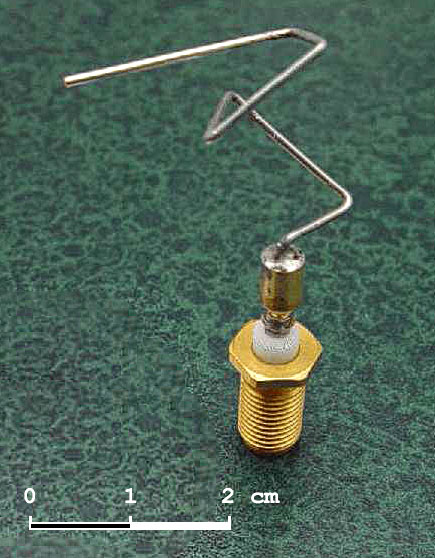
\includegraphics[width=\textwidth]{imagens/evolved_antenna.jpg}
        \caption{A antena evoluída, assim chamada por ter seu formato calculado por meio de um AG.}
      \end{figure}
    \end{column}
  \end{columns}
\end{frame}

\begin{frame}{Motivação}
  \begin{block}{Métodos para Otimização Numérica}
    \vfill
    \begin{itemize}
      \item Baseados em Cálculo
            \begin{itemize}
              \item Indiretos $\rightarrow$ Solução de $\nabla f = 0$
              \item Diretos $\rightarrow$ Procuram extremos escalando na direção de $\nabla f$.
                    Conhecidos por escalada de morro, ou \textit{hill climbing}
            \end{itemize}
      \item Enumerativos $\rightarrow$ Iteração sobre os membros de um espaço de busca finito,
            ou um espaço discreto infinito
      \item Procura Aleatória $\rightarrow$ \textit{Random walks}
    \end{itemize}
  \end{block}
\end{frame}

\begin{frame}{Um Exemplo}
  \begin{columns}
    \begin{column}{0.6\textwidth}
      Otimização numérica da função
      $$ f(x,y) = \cos(n\pi r)\exp\left(-\frac{r^2}{\sigma^2}\right) $$
      \begin{itemize}
        \item Sabemos que exitem máximos em $ \nicefrac{2k}{n} \text{ com } k \in \N $
        \item O máximo global ocorre quando $ k = 0 $
      \end{itemize}
    \end{column}
    \begin{column}{0.4\textwidth}
      \begin{figure}
        \centering
        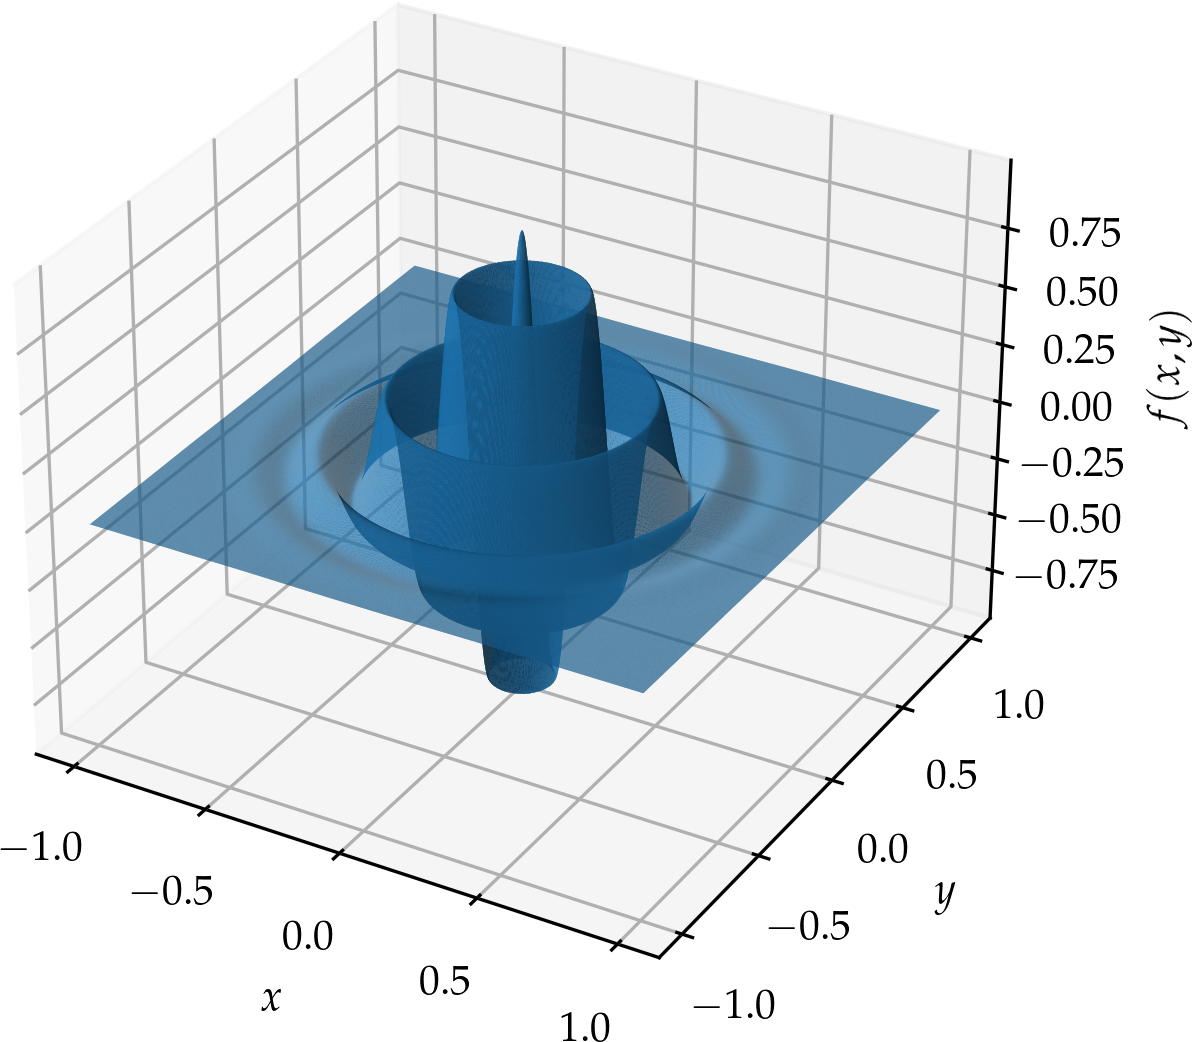
\includegraphics[width=\textwidth]{imagens/damped_cossine.png}
        \caption{Gráfico de $f(x, y)$ com $n = 9$ e $\sigma = 0,4$}
      \end{figure}
    \end{column}
  \end{columns}
\end{frame}

\begin{frame}{Um Exemplo}
  \begin{itemize}
    \item Algoritmos do tipo \textit{hill climbing} só teriam sucesso em
          $r < \nicefrac{1}{n}$, em $\approx 1\%$ das vezes, no caso ilustrado
    \item Os máximos locais atuariam como barreiras protegendo o máximo local
  \end{itemize}
  \vfill
  \begin{block}{}
    Como criar um algoritmo para otimização numérica que contorna essas dificuldades?
  \end{block}
\end{frame}

\begin{frame}{O Algoritmo Genético}
  \begin{block}{Vantagens}
    \vfill
    \begin{itemize}
      \item Não é limitado por restrições no espaço de busca\trav
            não depende da existência de derivada ou continuidade.
      \item A função objetivo pode ser aleatória ou mesmo depender do tempo
      \item É facilmente paralelizável
      \item São simples, do ponto de vista computacional
      \item Permite o mapeamento também dos máximos locais
    \end{itemize}
  \end{block}
\end{frame}

\begin{frame}{O Algoritmo Genético}
  \begin{block}{Em que consiste um AG?}
    \vfill
    \begin{itemize}
      \item Codificação da informação de um elemento do espaço de busca
            em um número de cromossomos
      \item Um conjunto de cromossomos qualifica um indivíduo
      \item Esses cromossomos são compostos por um número de genes,
            que podem ter como valores os alelos 0 ou 1
      \item Um conjunto de indivíduos similares qualifica uma população
    \end{itemize}
  \end{block}
\end{frame}

\begin{frame}{O Algoritmo Genético}
  \begin{block}{Em que consiste um AG?}
    \begin{itemize}
      \item Um mecanismo de seleção probabilístico escolhe um grupo
            de indivíduos
      \item A população evolui com a recombinação desses indivíduos
      \item Nesse processo, existe uma probabilidade de mutação nos genes
      \item A tendência será de que, após um longo período, os melhores
            indivíduos da população representem a solução do problema
    \end{itemize}
  \end{block}
\end{frame}

\begin{frame}{O Algoritmo Genético}
  \begin{figure}
  \centering
  \resizebox{\textwidth}{!}{
    \begin{tikzpicture}
      \node[start_end] (start) {Início};
      \node[process, right=1em of start] (init_pop) {População\\ Inicial};
      \node[process, right=1em of init_pop]  (selection) {Seleção};
      \node[process, below=1em of selection]  (crossover) {Recombinação};
      \node[process, below=1em of crossover]  (mutation) {Mutação};
      \node[decision, below=1em of mutation]  (check) {Condição atingida?};
      \node[start_end, left=10ex of check] (end) {Fim};
      \draw[myarrow=.9] (start.east) --  (init_pop.west);
      \draw[myarrow=.9] (init_pop.east) --  (selection.west);
      \draw[myarrow=.9] (selection.south) --  (crossover.north);
      \draw[myarrow=.9] (crossover.south) --  (mutation.north);
      \draw[myarrow=.9] (mutation.south) -- (check.north);
      \draw[myarrow=.9] (check.east) -- node[description, above] {Não} ([xshift=10ex]check.east) |- (selection.east);
      \draw[myarrow=.9] (check.west) -- node[description, above] {Sim} (end.east);
    \end{tikzpicture}
  }
  \caption{\textit{Flowchart} geral de um algoritmo genético.}
\end{figure}
\end{frame}

\section{Metodologia}

\newcommand{\kth}[2]{{#1}^{(k)}_{#2}}
\newcommand{\kpth}[2]{{#1}^{(k + 1)}_{#2}}
\newcommand{\xmin}[1]{x^{(min)}_{#1}}
\newcommand{\xmax}[1]{x^{(max)}_{#1}}

\begin{frame}{Codificação}
  Vamos considerar uma função objetivo $ f : \mathcal{C} \subseteq \R^m \rightarrow \R $
  \begin{itemize}
    \item A população é representada por $n$ matrizes
          $$
            A_k = \left[
              \begin{matrix}
                \kth{a}{11} & \cdots & \kth{a}{1m} \\
                \vdots      & \ddots & \vdots      \\
                \kth{a}{l1} & \cdots & \kth{a}{lm} \\
              \end{matrix}
              \right]
          $$
    \item As respectivas $n$ posições são
          $$ X_k = \left( \kth{x}{1}, \mathdots, \; \kth{x}{j}, \mathdots, \; \kth{x}{m} \right) $$
  \end{itemize}
\end{frame}

\begin{frame}{Codificação}
  \begin{itemize}
    \item O espaço de busca é $S \subseteq \mathcal{C}$ tal que
          $$ \mathcal{S} = \bigtimes_{j = 1}^m \; [ \xmin{j} \; , \; \xmax{j} ] $$
    \item $l$ bits representam inteiros em $ [0, 2^l - 1) $
    \item As posições são obtidas dos cromossomos por
          $$ x^{(k)}_j = \xmin{j} + \frac{\xmax{j} - \xmin{j}}{2^l - 1} \sum_{i = 1}^l \kth{a}{ij} 2^{i - 1} $$
  \end{itemize}
\end{frame}

\begin{frame}{Codificação}
  \begin{itemize}
    \item A relação inversa é obtida por
          $$
            \sum_{i = 1}^l \kth{a}{ij} 2^{i - 1} =
            \left\lfloor \frac{(\kth{x}{j} - \xmin{j})(2^l - 1)}{\xmax{j} - \xmin{j}} \right\rfloor
          $$
  \end{itemize}
\end{frame}

\newcommand{\fmin}{f_{min}}
\newcommand{\fmax}{f_{max}}

\begin{frame}{Seleção}
  \begin{itemize}
    \item Função Desempenho $g : \R \rightarrow \R$ tal que
          $$ P_k = \frac{g(f(X_k))}{\sum_{j = 1}^n g(f(X_j))} $$
    \item A função usada foi um escalamento linear $$ g(x) = ax + b $$
          $$
            a =
            \begin{cases}
              \frac{\mu (h - 1)}{\fmax - \mu} \;, & \text{se } \fmin > \frac{h\mu - \fmax}{h - 1} \\
              \frac{\mu}{\mu - \fmin}         \;, & \text{caso contrário}
            \end{cases}
          $$
          $$
            b =
            \begin{cases}
              \frac{\mu (\fmax - h\mu)}{\fmax - \mu} \;, & \text{se } \fmin > \frac{h\mu - \fmax}{h - 1} \\
              - \frac{\mu\fmin}{\mu - \fmin}         \;, & \text{caso contrário}
            \end{cases}
          $$
  \end{itemize}
\end{frame}

\begin{frame}{Seleção}
  \begin{itemize}
    \item Caso $g(f(X_k)) < 0$ para algum $k$, fazemos $g = 0$
          para os indivíduos correspondentes
    \item É feito o sorteio de $\nicefrac{n}{2}$ indivíduos por meio de
          uma roleta simples
    \item Os indivíduos selecionados são
          $$ S = \left\{ S_1\;, \mathdots,  \;S_k\;, \mathdots, \;S_{\nicefrac{n}{2}} \right\} $$
  \end{itemize}
  \vfill
  \begin{block}{Motivos para essa escolha de $g$}
    \begin{itemize}
      \item Evita a convergência prematura da população
      \item Aumenta a variabilidade genética
      \item Aumenta a probabilidade de que vários máximos locais coexistam
            na população com o máximo global
    \end{itemize}
  \end{block}
\end{frame}

\begin{frame}{Recombinação e Mutação}
  \begin{itemize}
    \item Cada cromossomo terá dois pontos de recombinação
    \item Sorteio de $ \kth{\alpha}{j} $ e $ \kth{\beta}{j} $ tais que
          $ 0 \leq \kth{\alpha}{j} < \kth{\beta}{j} $ e $ \kth{\alpha}{j} \leq \kth{\beta}{j} < l $ onde
          $ j = 0, 1, \dots, m $ e $ k = 0, 2, 4, \dots, \nicefrac{n}{2} - 2 $
    \item Com esses valores, criamos a máscara de combinação
          $$
            \kth{r}{ij} =
            \begin{cases}
              0 \;, & \text{se } i \leq \kth{\alpha}{j} \text{ ou } i > \kth{\beta}{j} \\
              1 \;, & \text{caso contrário}
            \end{cases}
          $$
    \item Criamos uma máscara de mutação
          $$
            \kth{m}{ij} =
            \begin{cases}
              1 \;, & \text{se houver mutação} \\
              0 \;, & \text{caso contrário}
            \end{cases}
          $$
  \end{itemize}
\end{frame}

\begin{frame}{Recombinação e Mutação}
  \begin{itemize}
    \item O conjunto dos indivíduos filhos será
          $$ S' = \left\{ S'_1\;, \mathdots,  \;S'_k\;, \mathdots, \;S'_{\nicefrac{n}{2}} \right\} $$
          $$ \kth{s'}{ij} = (\kth{s}{ij} \land \kth{r}{ij}) \lor (\kpth{s}{ij} \land \lnot \kth{r}{ij}) \oplus \kth{m}{ij} $$
          $$ \kpth{s'}{ij} = (\kth{s}{ij} \land \lnot \kth{r}{ij}) \lor (\kpth{s}{ij} \land \kth{r}{ij}) \oplus \kth{m}{ij} $$
    \item A população da geração seguinte é $ S \cup S' $
  \end{itemize}
\end{frame}

\begin{frame}{Recombinação e Mutação}
  \begin{figure}
  \centering
  \resizebox*{\textwidth}{!}{
    \begin{tikzpicture}
      \def\verticalmargin{1.3}
      \begin{scope}[local bounding box=fig1]
        \begin{scope}[start chain=1 going right,node distance=-0.15mm]
          \node [on chain=1,gene] (parent_1_left)     {0};
          \node [on chain=1,gene] (recomb_point_1_up) {0};
          \node [on chain=1,gene_filled]              {1};
          \node [on chain=1,gene_filled]              {0};
          \node [on chain=1,gene_filled]              {1};
          \node [on chain=1,gene_filled]              {1};
          \node [on chain=1,gene] (recomb_point_2_up) {0};
          \node [on chain=1,gene] (parent_1_right)    {1};
          \node [left=of parent_1_left] {$S_k$};
        \end{scope}
        \begin{scope}[start chain=1 going right,node distance=-0.15mm, shift={(0,-\verticalmargin)}]
          \node [on chain=1,gene] (mask_left)  {0};
          \node [on chain=1,gene]              {0};
          \node [on chain=1,gene]              {1};
          \node [on chain=1,gene]              {1};
          \node [on chain=1,gene]              {1};
          \node [on chain=1,gene]              {1};
          \node [on chain=1,gene]              {0};
          \node [on chain=1,gene] (mask_right) {0};
          \node [left=of mask_left] {$R$};
        \end{scope}
        \begin{scope}[start chain=1 going right,node distance=-0.15mm, shift={(0,-2*\verticalmargin)}]
          \node [on chain=1,gene_filled] (parent_2_left)       {1};
          \node [on chain=1,gene_filled] (recomb_point_1_down) {1};
          \node [on chain=1,gene]                              {1};
          \node [on chain=1,gene]                              {1};
          \node [on chain=1,gene]                              {1};
          \node [on chain=1,gene]                              {0};
          \node [on chain=1,gene_filled] (recomb_point_2_down) {1};
          \node [on chain=1,gene_filled] (parent_2_right)      {0};
          \node [left=of parent_2_left] {$S_{k + 1}$};
        \end{scope}
        \begin{scope}[start chain=1 going right,node distance=-0.15mm, shift={(0,-3*\verticalmargin)}]
          \node [on chain=1,gene_mutated] (mutation_left) {1};
          \node [on chain=1,gene]                         {0};
          \node [on chain=1,gene]                         {0};
          \node [on chain=1,gene]                         {0};
          \node [on chain=1,gene]                         {0};
          \node [on chain=1,gene]                         {0};
          \node [on chain=1,gene]                         {0};
          \node [on chain=1,gene]                         {0};
          \node [left=of mutation_left] {$M$};
        \end{scope}
        \draw ($(fig1.north west)+(0,0.85)$) rectangle ($(fig1.south east)+(0.15,-0.15)$);
        \draw [densely dotted] (recomb_point_1_up.east) -- (recomb_point_1_down.east);
        \draw [densely dotted] (recomb_point_2_up.west) -- (recomb_point_2_down.west);
        \node [description, font=\tiny, above=1.5ex of recomb_point_1_up.east] {Ponto de\\ Recombinação};
      \end{scope}
      \begin{scope}[xshift=22em, local bounding box=fig2]
        \begin{scope}[start chain=1 going right,node distance=-0.15mm]
          \node [on chain=1,gene_mutated] (mut_offspring_1_left) {1};
          \node [on chain=1,gene]                                {0};
          \node [on chain=1,gene]                                {1};
          \node [on chain=1,gene]                                {1};
          \node [on chain=1,gene]                                {1};
          \node [on chain=1,gene]                                {0};
          \node [on chain=1,gene]                                {0};
          \node [on chain=1,gene] (mut_offspring_1_right)        {1};
        \end{scope}
        \begin{scope}[start chain=1 going right,node distance=-0.15mm, shift={(0,-1*\verticalmargin)}]
          \node [on chain=1,gene] (offspring_1_left)  {0};
          \node [on chain=1,gene]                     {0};
          \node [on chain=1,gene]                     {1};
          \node [on chain=1,gene]                     {1};
          \node [on chain=1,gene]                     {1};
          \node [on chain=1,gene]                     {0};
          \node [on chain=1,gene]                     {0};
          \node [on chain=1,gene] (offspring_1_right) {1};
        \end{scope}
        \begin{scope}[start chain=1 going right,node distance=-0.15mm, shift={(0,-2*\verticalmargin)}]
          \node [on chain=1,gene_filled] (offspring_2_left)  {1};
          \node [on chain=1,gene_filled]                     {1};
          \node [on chain=1,gene_filled]                     {1};
          \node [on chain=1,gene_filled]                     {0};
          \node [on chain=1,gene_filled]                     {1};
          \node [on chain=1,gene_filled]                     {1};
          \node [on chain=1,gene_filled]                     {1};
          \node [on chain=1,gene_filled] (offspring_2_right) {0};
        \end{scope}
        \begin{scope}[start chain=1 going right,node distance=-0.15mm, shift={(0,-3*\verticalmargin)}]
          \node [on chain=1,gene_mutated] (mut_offspring_2_left) {0};
          \node [on chain=1,gene_filled]                         {1};
          \node [on chain=1,gene_filled]                         {1};
          \node [on chain=1,gene_filled]                         {0};
          \node [on chain=1,gene_filled]                         {1};
          \node [on chain=1,gene_filled]                         {1};
          \node [on chain=1,gene_filled]                         {1};
          \node [on chain=1,gene_filled] (mut_offspring_2_right) {0};
        \end{scope}
        \path [font=\tiny] (mask_right.east)++(0.15,0) edge node [above] {$(S_k \land R ) \lor (S_{k + 1} \land \lnot R)$} (offspring_1_left.west);
        \path [font=\tiny] (parent_2_right.east)++(0.15,0) edge node [below] {$(S_k \land \lnot R ) \lor (S_{k + 1} \land R)$} (offspring_2_left.west);
        \path [font=\tiny] (offspring_1_right.east) edge[bend right=90] node [left] {$\oplus M$} (mut_offspring_1_right.east);
        \path [font=\tiny] (offspring_2_right.east) edge[bend left=90] node [left] {$\oplus M$} (mut_offspring_2_right.east);
      \end{scope}
    \end{tikzpicture}
  }
  \caption{
    Diagrama ilustrando\trav em um caso com $m = 1$ e $l = 8$\trav a recombinação entre os indivíduos $S_k$ e $S_{k + 1}$
    e mutação nos filhos gerados segundo as respectivas máscaras de recombinação e mutação $R$ e $M$.
  }
  \label{fig:recomb_diagram}
\end{figure}

\end{frame}

\begin{frame}{Estratégia Elitista}
  $$
    S =
    \left\{
    \underbrace{S_{\epsilon}\;, \mathdots,  \;S_{\epsilon}}_{e_1 \text{ cópias}}\;,\;
    \overbrace{S_{\epsilon}\;, \mathdots,  \;S_{\epsilon}}^{e_2 \text{ cópias}}\;,\;
    \underbrace{S_{e_1 + e_2 + 1}\;, \mathdots,  \;S_{\nicefrac{n}{2}}}_{\mathllap{e_3 \text{ cópias dentre os restantes}}}
    \right\}
  $$
  \begin{itemize}
    \item $S_\epsilon$ é o melhor indivíduo
    \item As primeiras $e_1$ cópias de $S_\epsilon$ terão probabilidade de mutação $p_1 = 0$
    \item As $e_2$ cópias de $S_\epsilon$ terão probabilidade de mutação $p_2$
    \item As $e_3$ cópias de $S_\epsilon$ terão probabilidade de mutação $p_3$
  \end{itemize}
\end{frame}

\begin{frame}{Estratégia Elitista}
  \begin{block}{Motivos para o uso de elitismo}
    \begin{itemize}
      \item Garante o $S_\epsilon$ na população seguinte
      \item Mutações de $S_\epsilon$ na geração seguinte
      \item Filhos de $S_\epsilon$ com outros membros da população
      \item Ganho de performance em funções comportadas
    \end{itemize}
  \end{block}
  \begin{alertblock}{Observação}
    \begin{itemize}
      \item Essa é apenas uma dentre muitas estratégias \cite{goldberg1989ga}
      \item Os parâmetros devem ser ajustados caso a caso
    \end{itemize}
  \end{alertblock}
\end{frame}

\section{Resultados}

\begin{frame}{Funções de Teste}
  \begin{columns}
    \begin{column}{0.5\textwidth}
      $$ f_1(x,y) = \cos(9\pi r)\exp\left\{-\frac{r^2}{(0,4)^2}\right\} $$
      $$ r = \sqrt{
          \left(x - 0,5\right)^2 +
          \left(y - 0,5\right)^2
        } $$
    \end{column}
    \begin{column}{0.5\textwidth}
      \begin{figure}
        \centering
        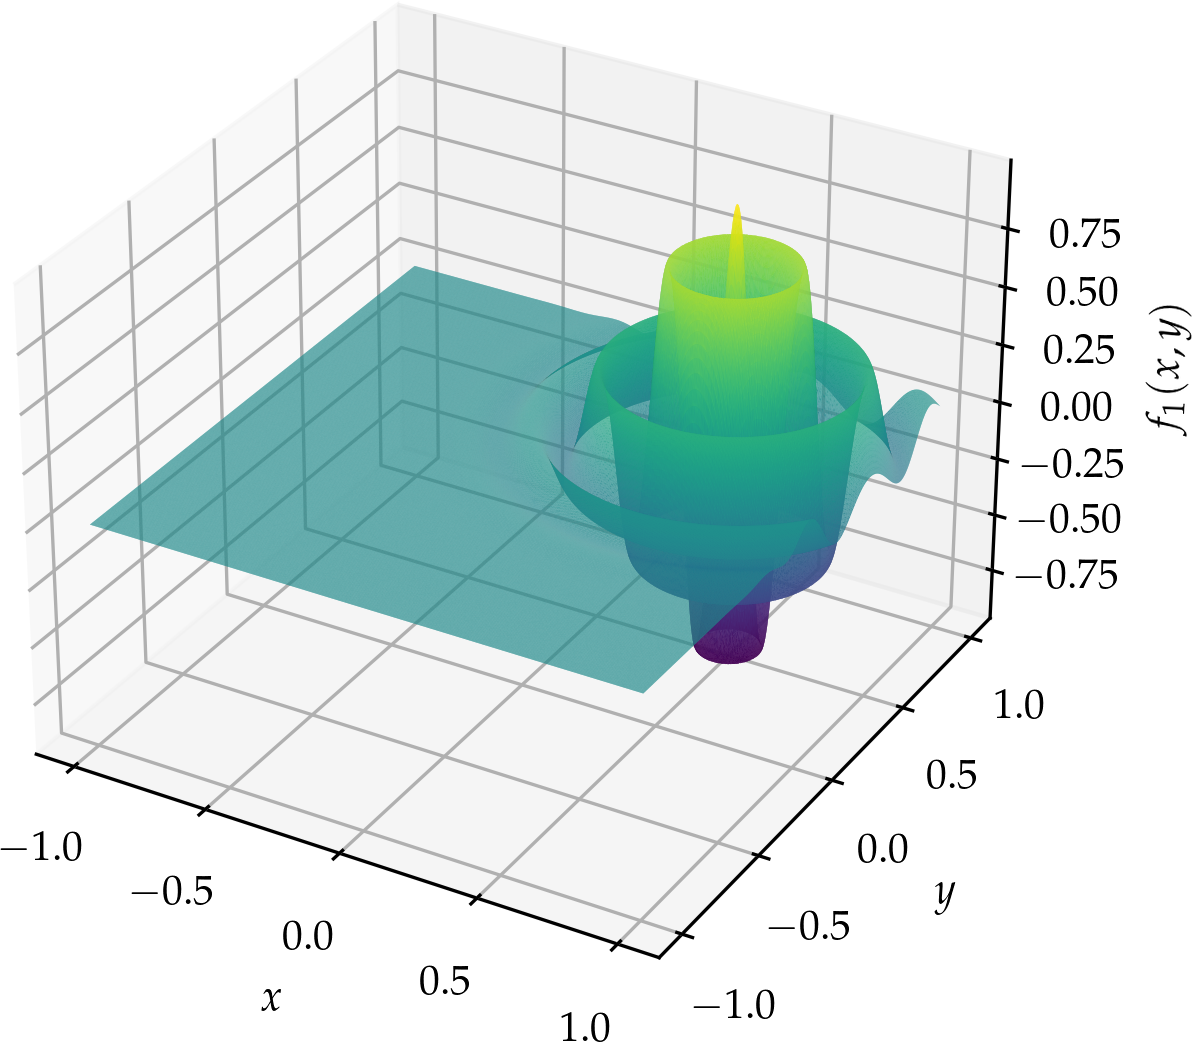
\includegraphics[width=\textwidth]{imagens/graph_damped_cossine.png}
        \caption{Gráfico de $f_1(x,y)$.}
      \end{figure}
    \end{column}
  \end{columns}
\end{frame}

\begin{frame}{Funções de Teste}
  \begin{columns}
    \begin{column}{0.5\textwidth}
      \begin{align*}
        \begin{split}
          & f_2(x,y) = \\
          & + 0,8 \exp\left\{-\frac{r_1^2}{(0,3)^2}\right\} \\
          & + 0,88 \exp\left\{-\frac{r_2^2}{(0,03)^2}\right\} \\
        \end{split}
      \end{align*}
      $$ r_1 = \sqrt{
          \left(x - 0,5\right)^2 +
          \left(y - 0,5\right)^2
        }
      $$
      $$ r_2 = \sqrt{
          \left(x - 0,6\right)^2 +
          \left(y - 0,1\right)^2
        }
      $$
    \end{column}
    \begin{column}{0.5\textwidth}
      \begin{figure}
        \centering
        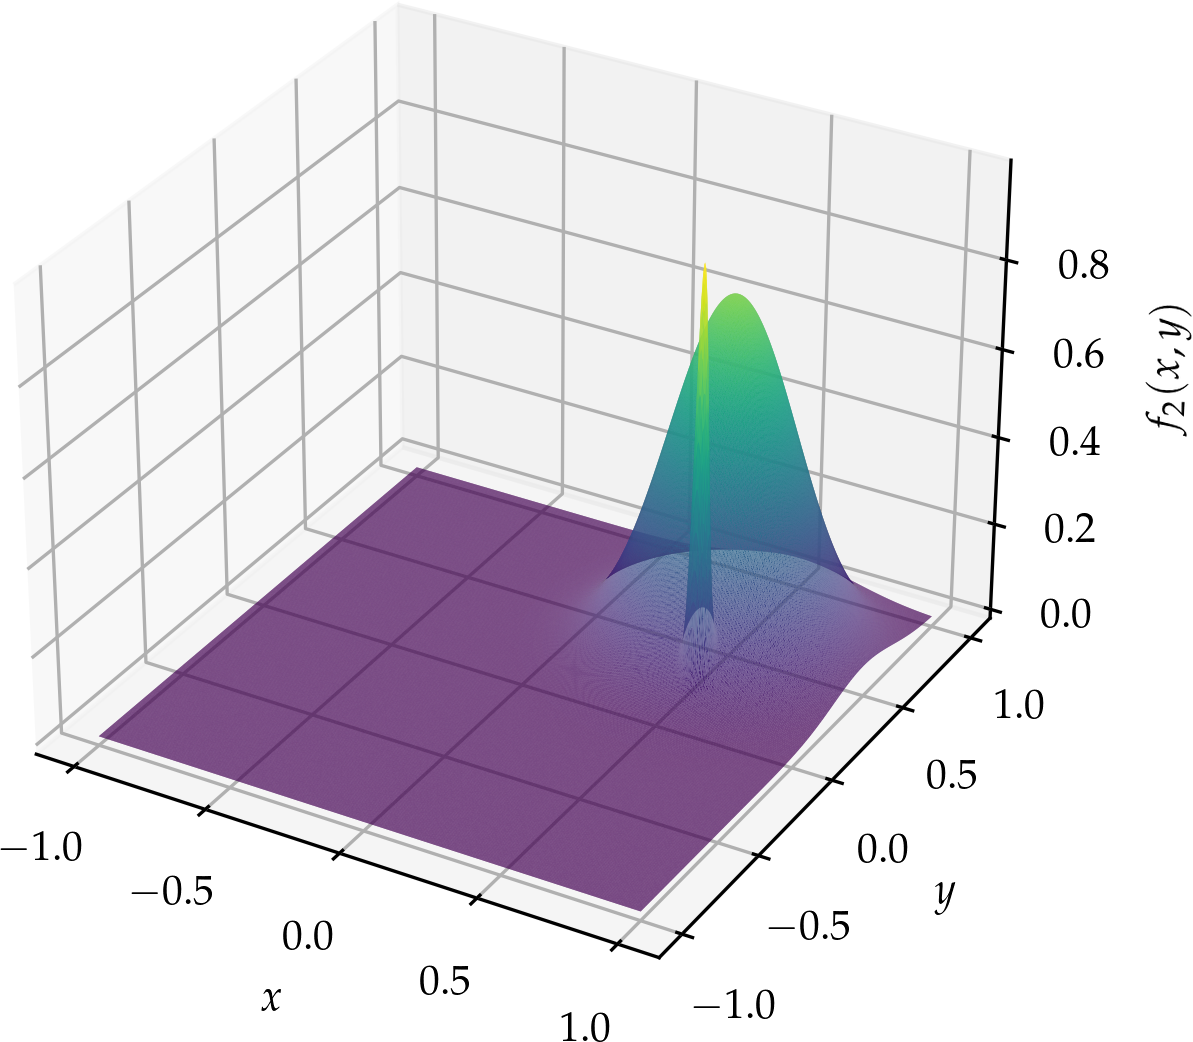
\includegraphics[width=\textwidth]{imagens/graph_near_gaussians.png}
        \caption{Gráfico de $f_2(x,y)$.}
      \end{figure}
    \end{column}
  \end{columns}
\end{frame}

\begin{frame}
  \begin{block}{Configurações Utilizadas}
    \begin{itemize}
      \item 8 populações de 1000 indivíduos
      \item Cromossomos de 32 bits
      \item Espaço de busca $\mathcal{S} = [-1,1] \times [-1,1]$
      \item Parâmetro da função desempenho $h = 2$
      \item $e_1 = 4$, $e_2 = 6$, $e_3 = 10$
      \item $p_2 = p_3 = 5\%$ e $p_2 = p_3 = 20\%$
    \end{itemize}
  \end{block}
\end{frame}

\begin{frame}
  \begin{figure}
    \centering
    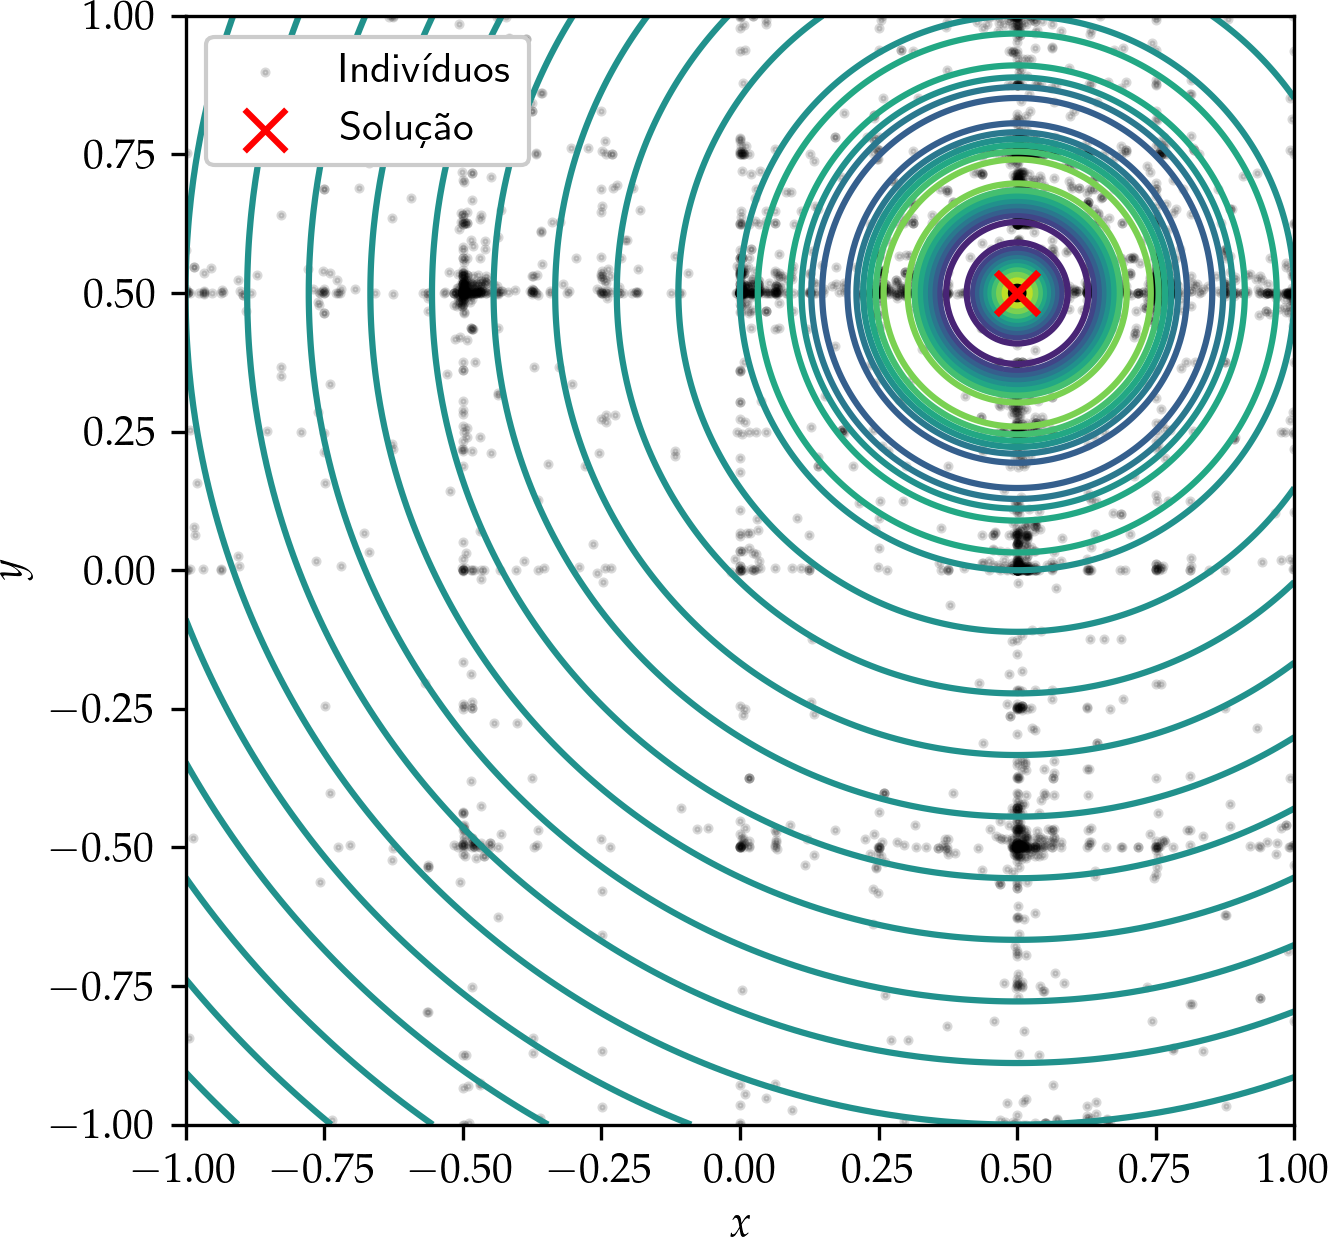
\includegraphics[height=0.95\textheight]{imagens/low_prob/contour_damped_cossine.png}
  \end{figure}
\end{frame}

\begin{frame}
  \begin{figure}
    \centering
    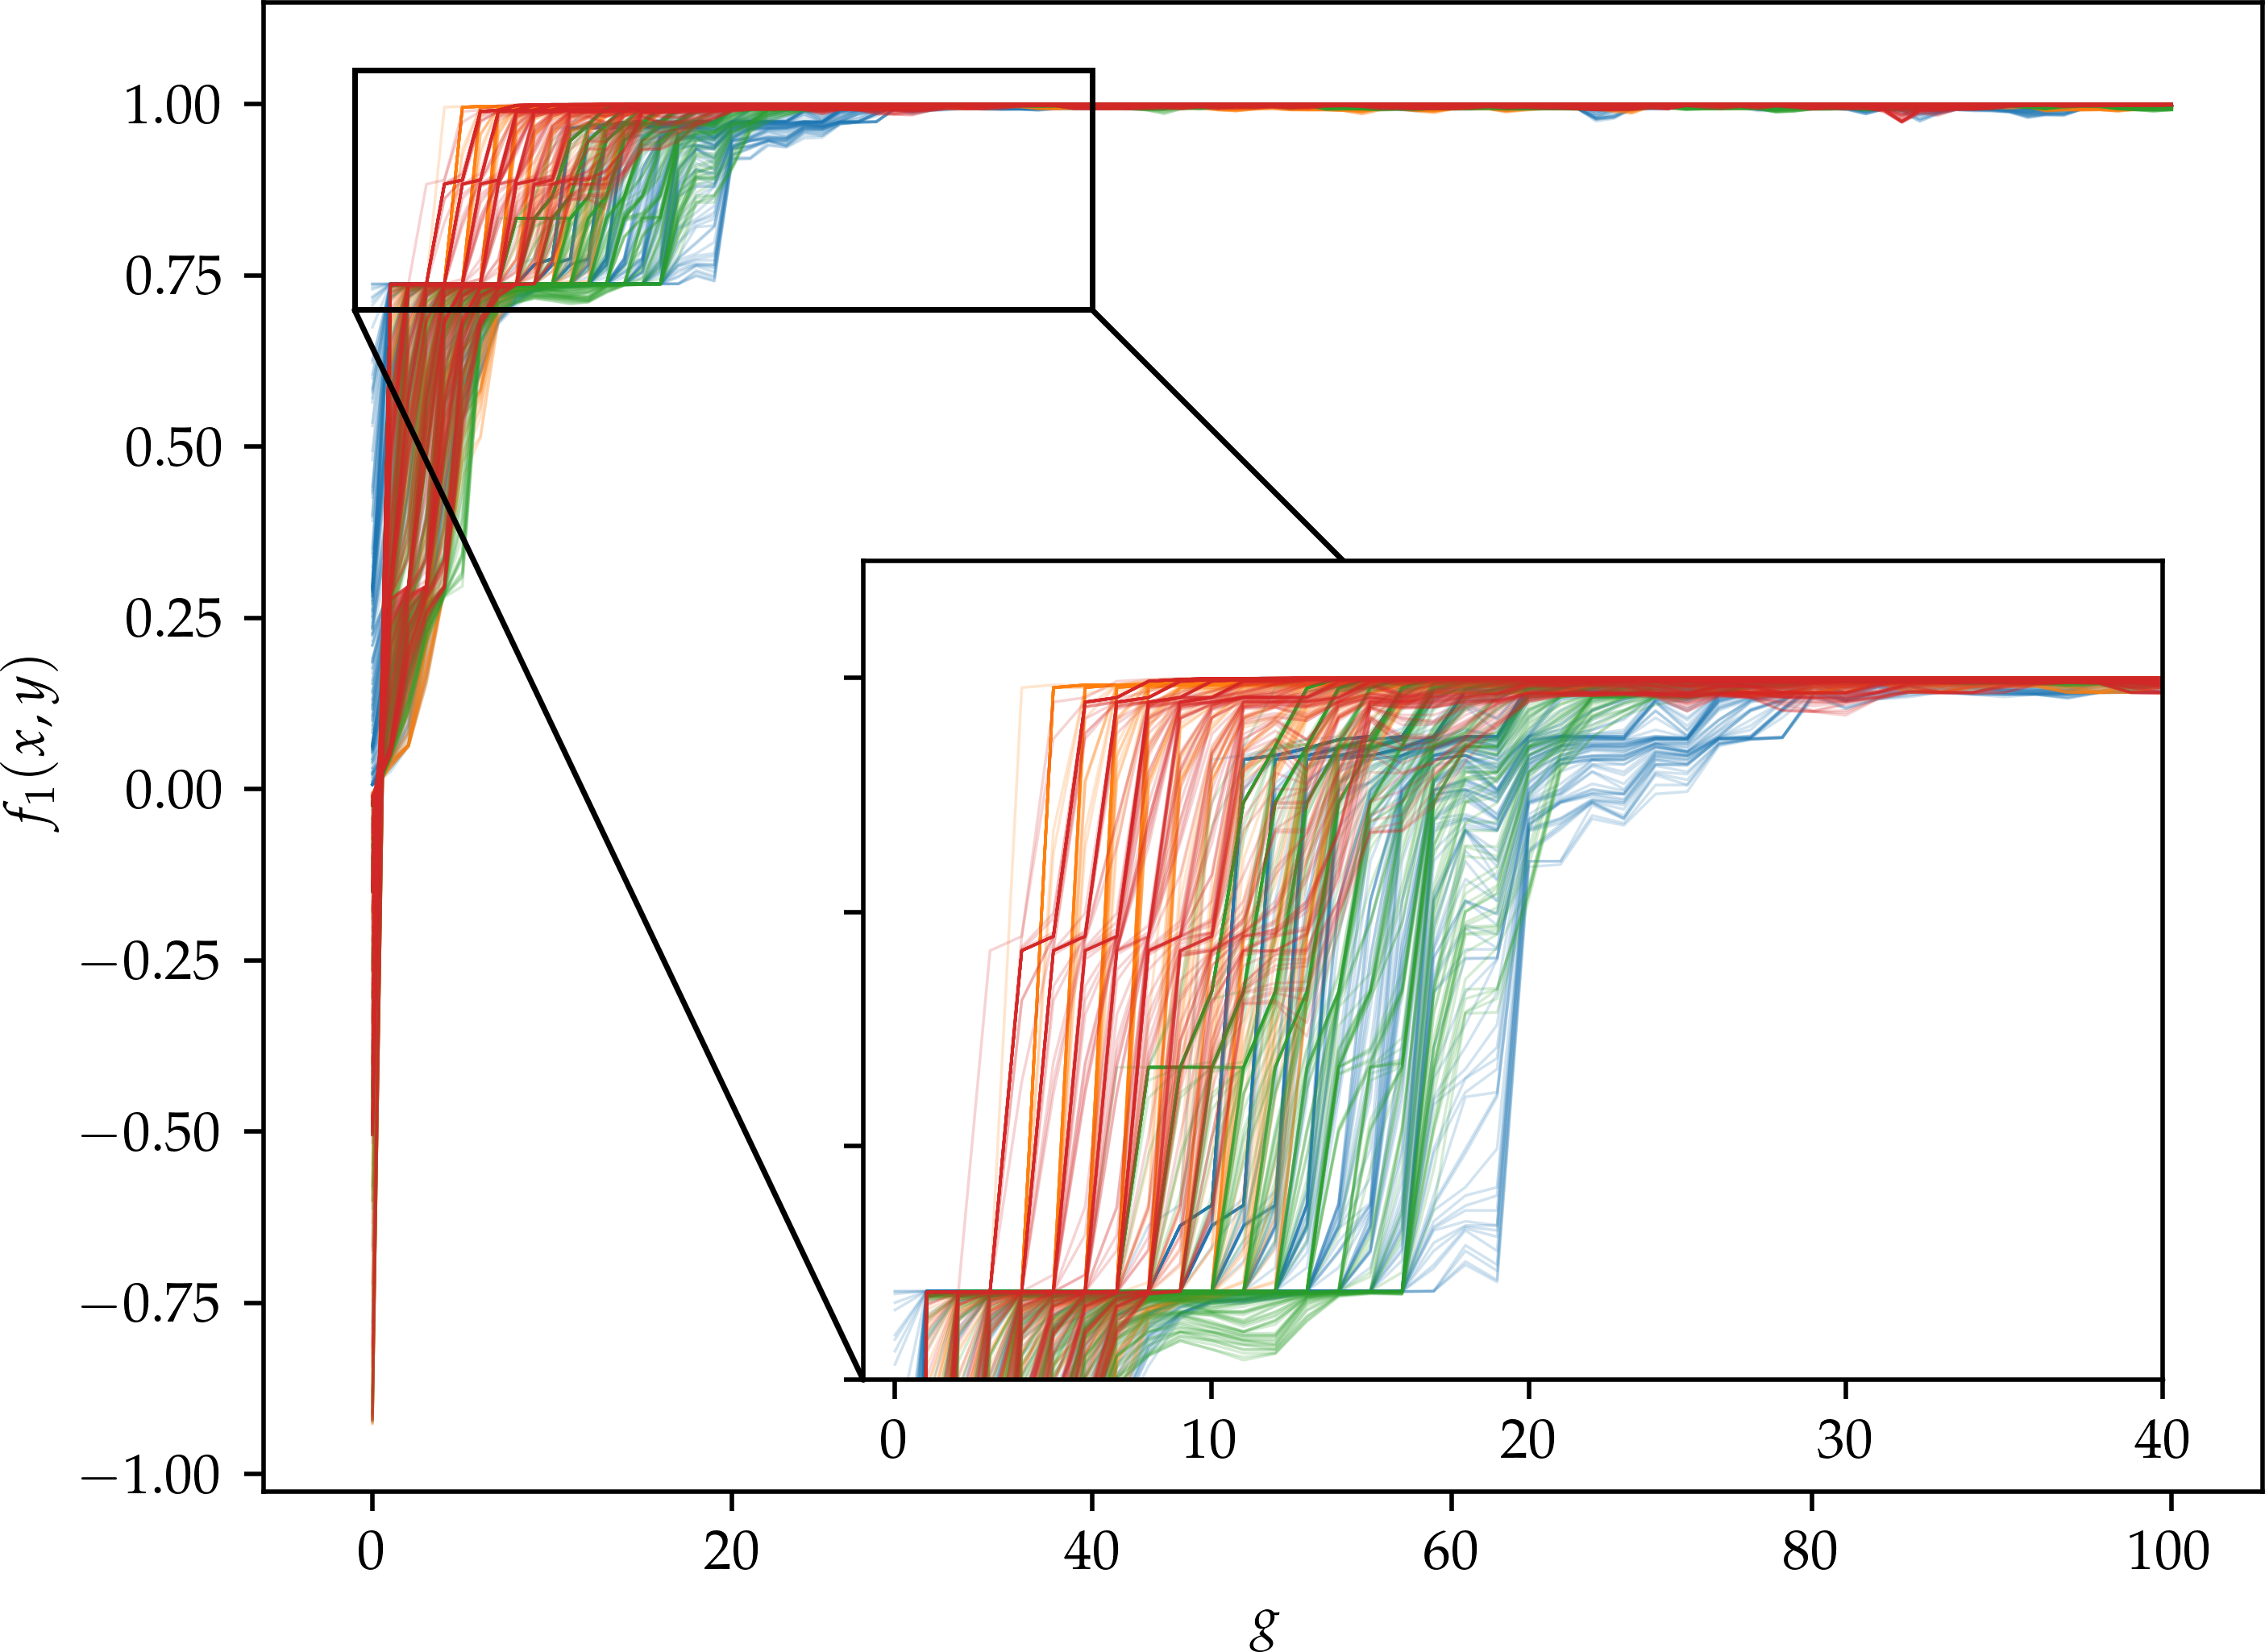
\includegraphics[height=0.95\textheight]{imagens/low_prob/evolution_damped_cossine.png}
  \end{figure}
\end{frame}

\begin{frame}
  \begin{figure}
    \centering
    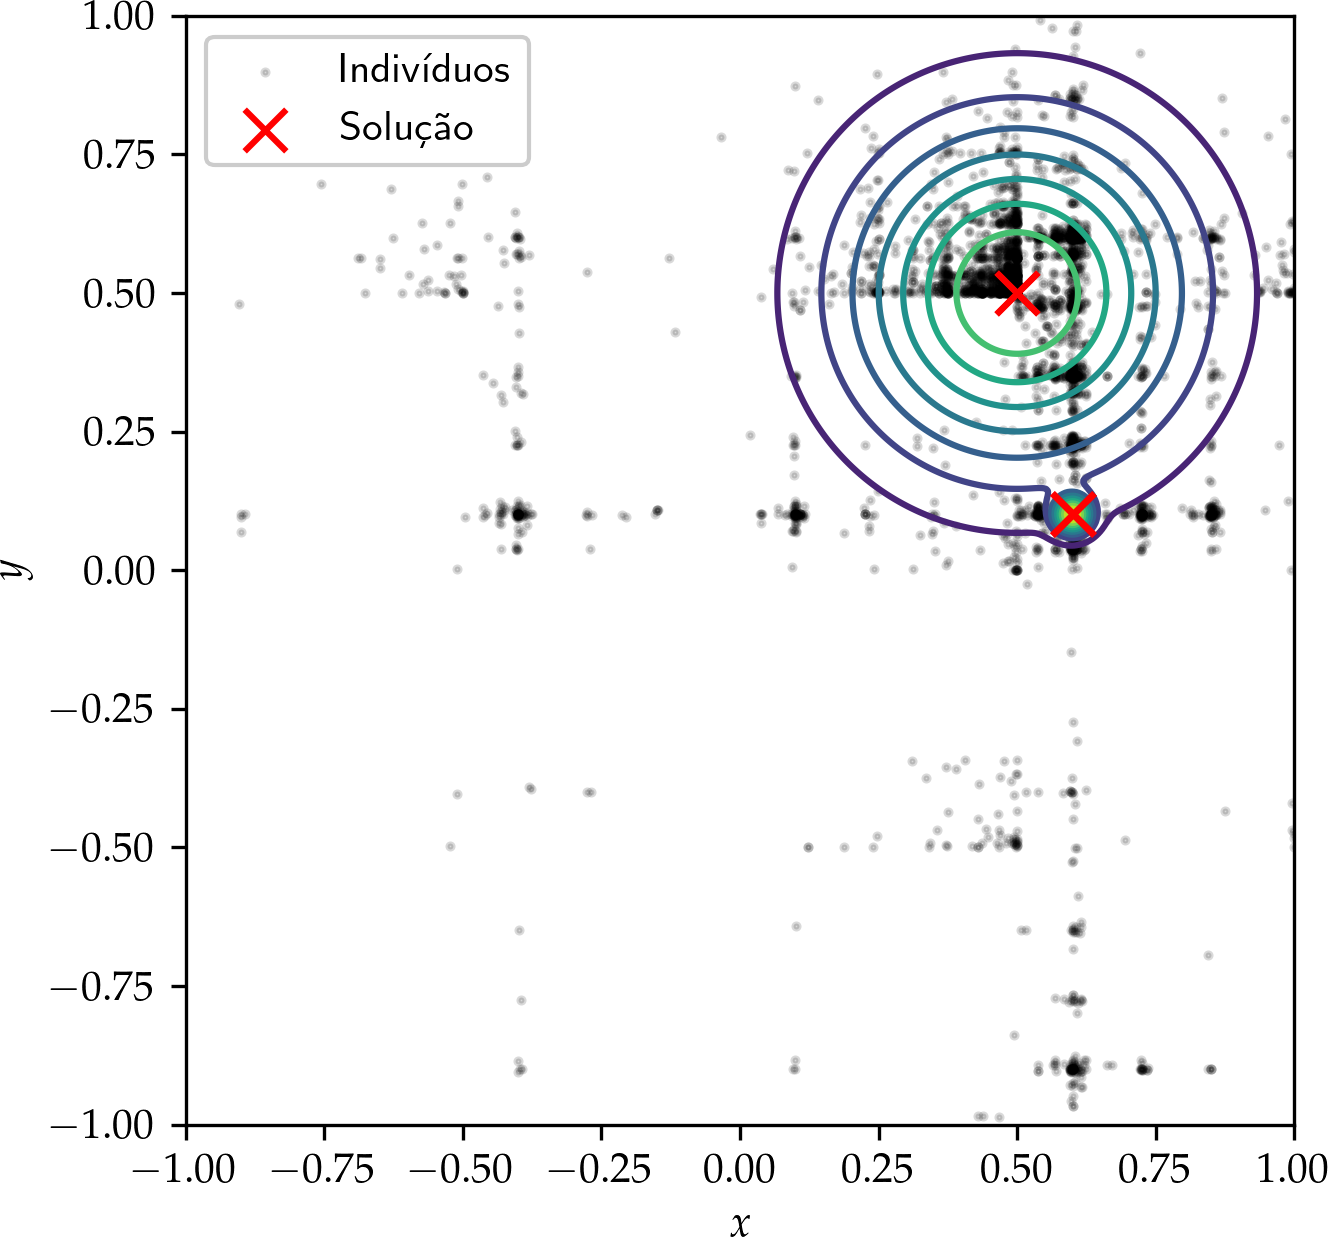
\includegraphics[height=0.95\textheight]{imagens/low_prob/contour_near_gaussians.png}
  \end{figure}
\end{frame}

\begin{frame}
  \begin{figure}
    \centering
    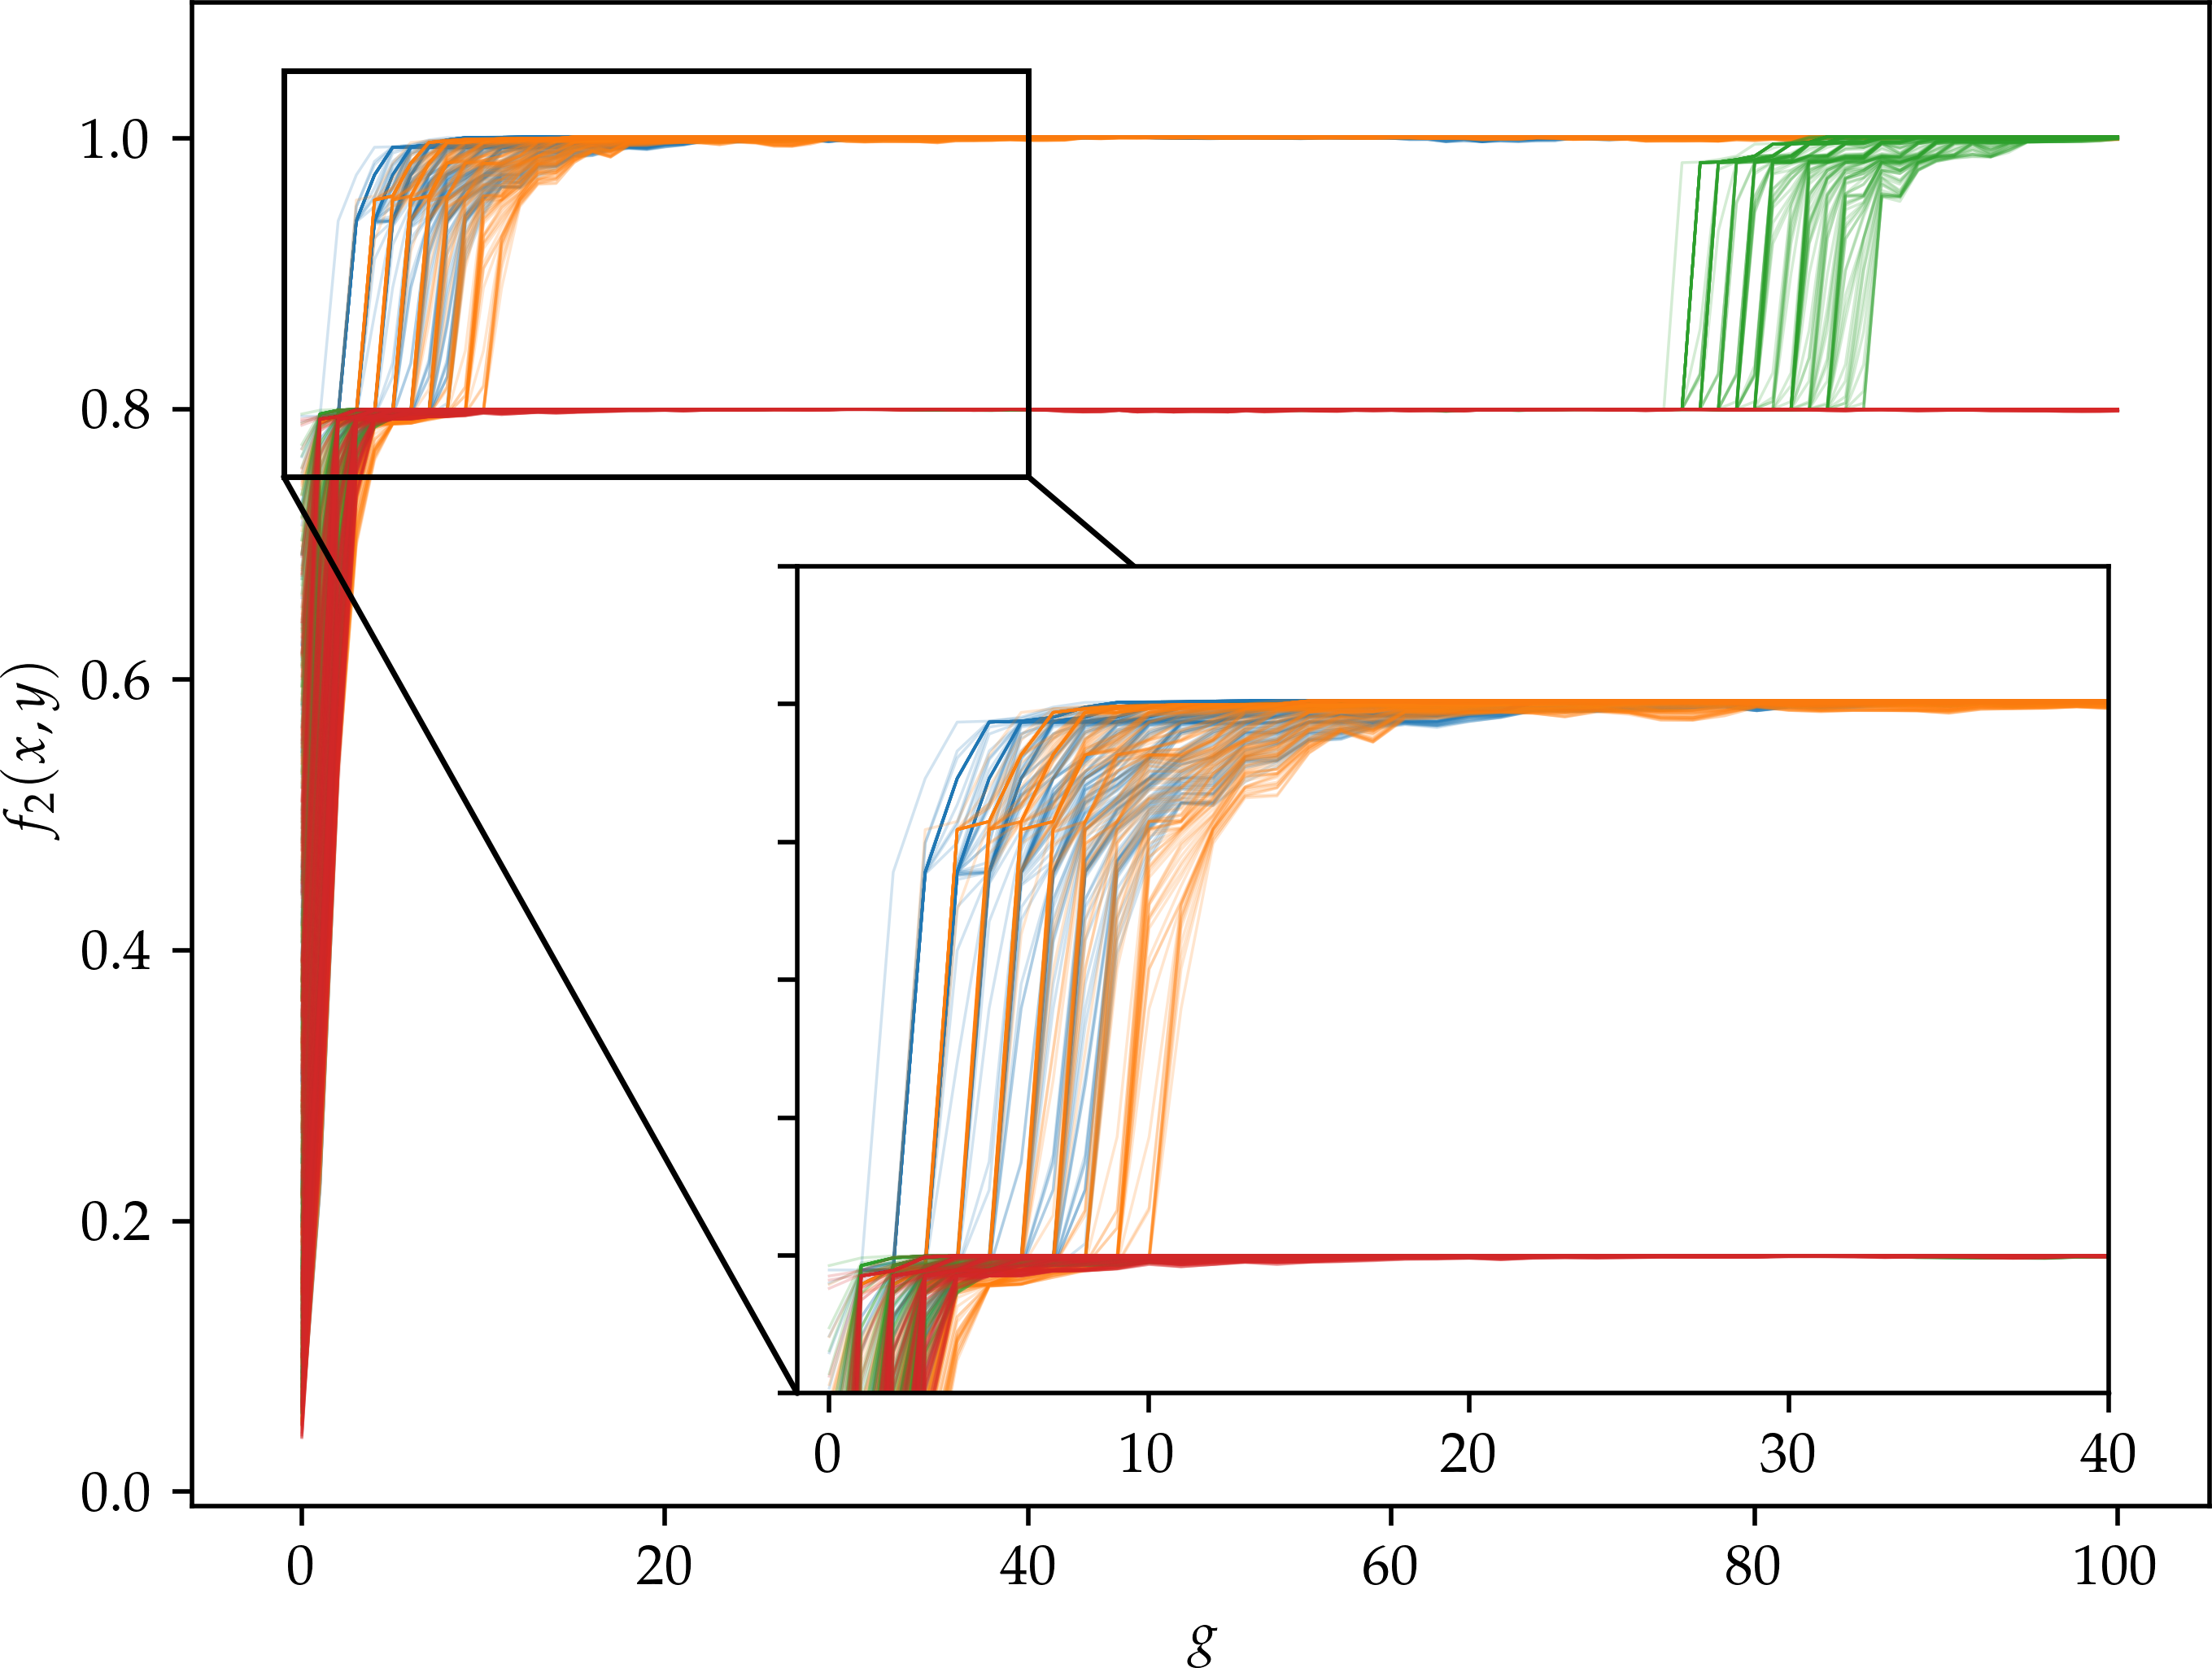
\includegraphics[height=0.95\textheight]{imagens/low_prob/evolution_near_gaussians.png}
  \end{figure}
\end{frame}

\begin{frame}
  \begin{figure}
    \centering
    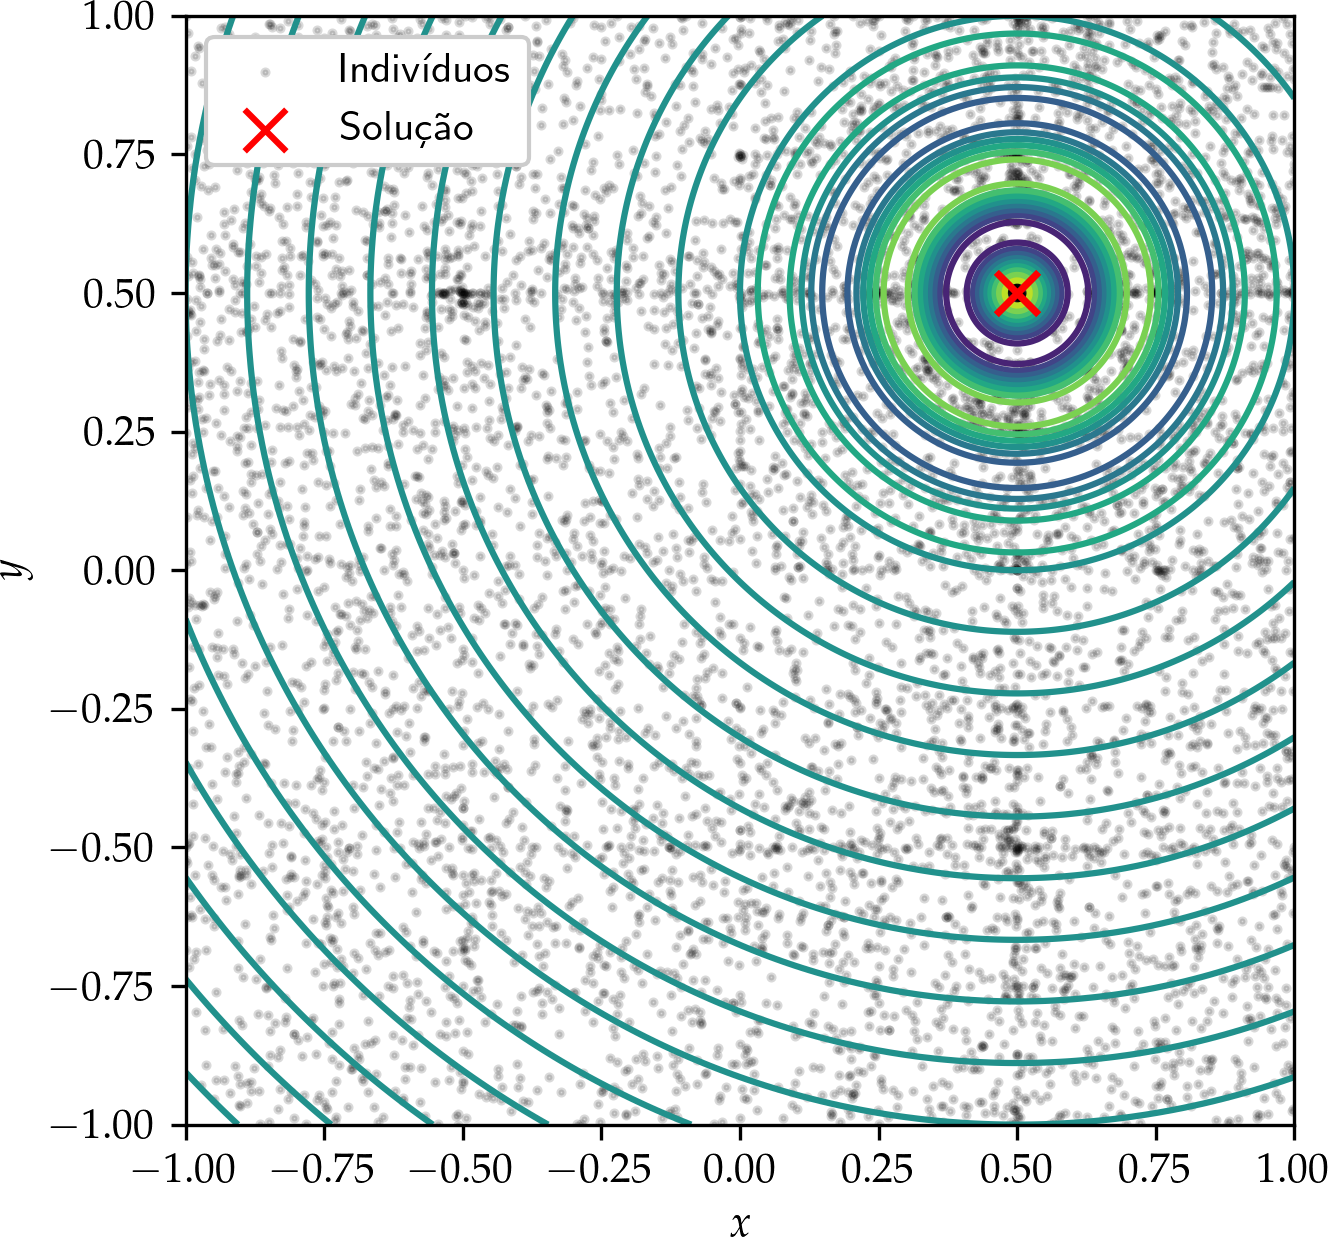
\includegraphics[height=0.95\textheight]{imagens/high_prob/contour_damped_cossine.png}
  \end{figure}
\end{frame}

\begin{frame}
  \begin{figure}
    \centering
    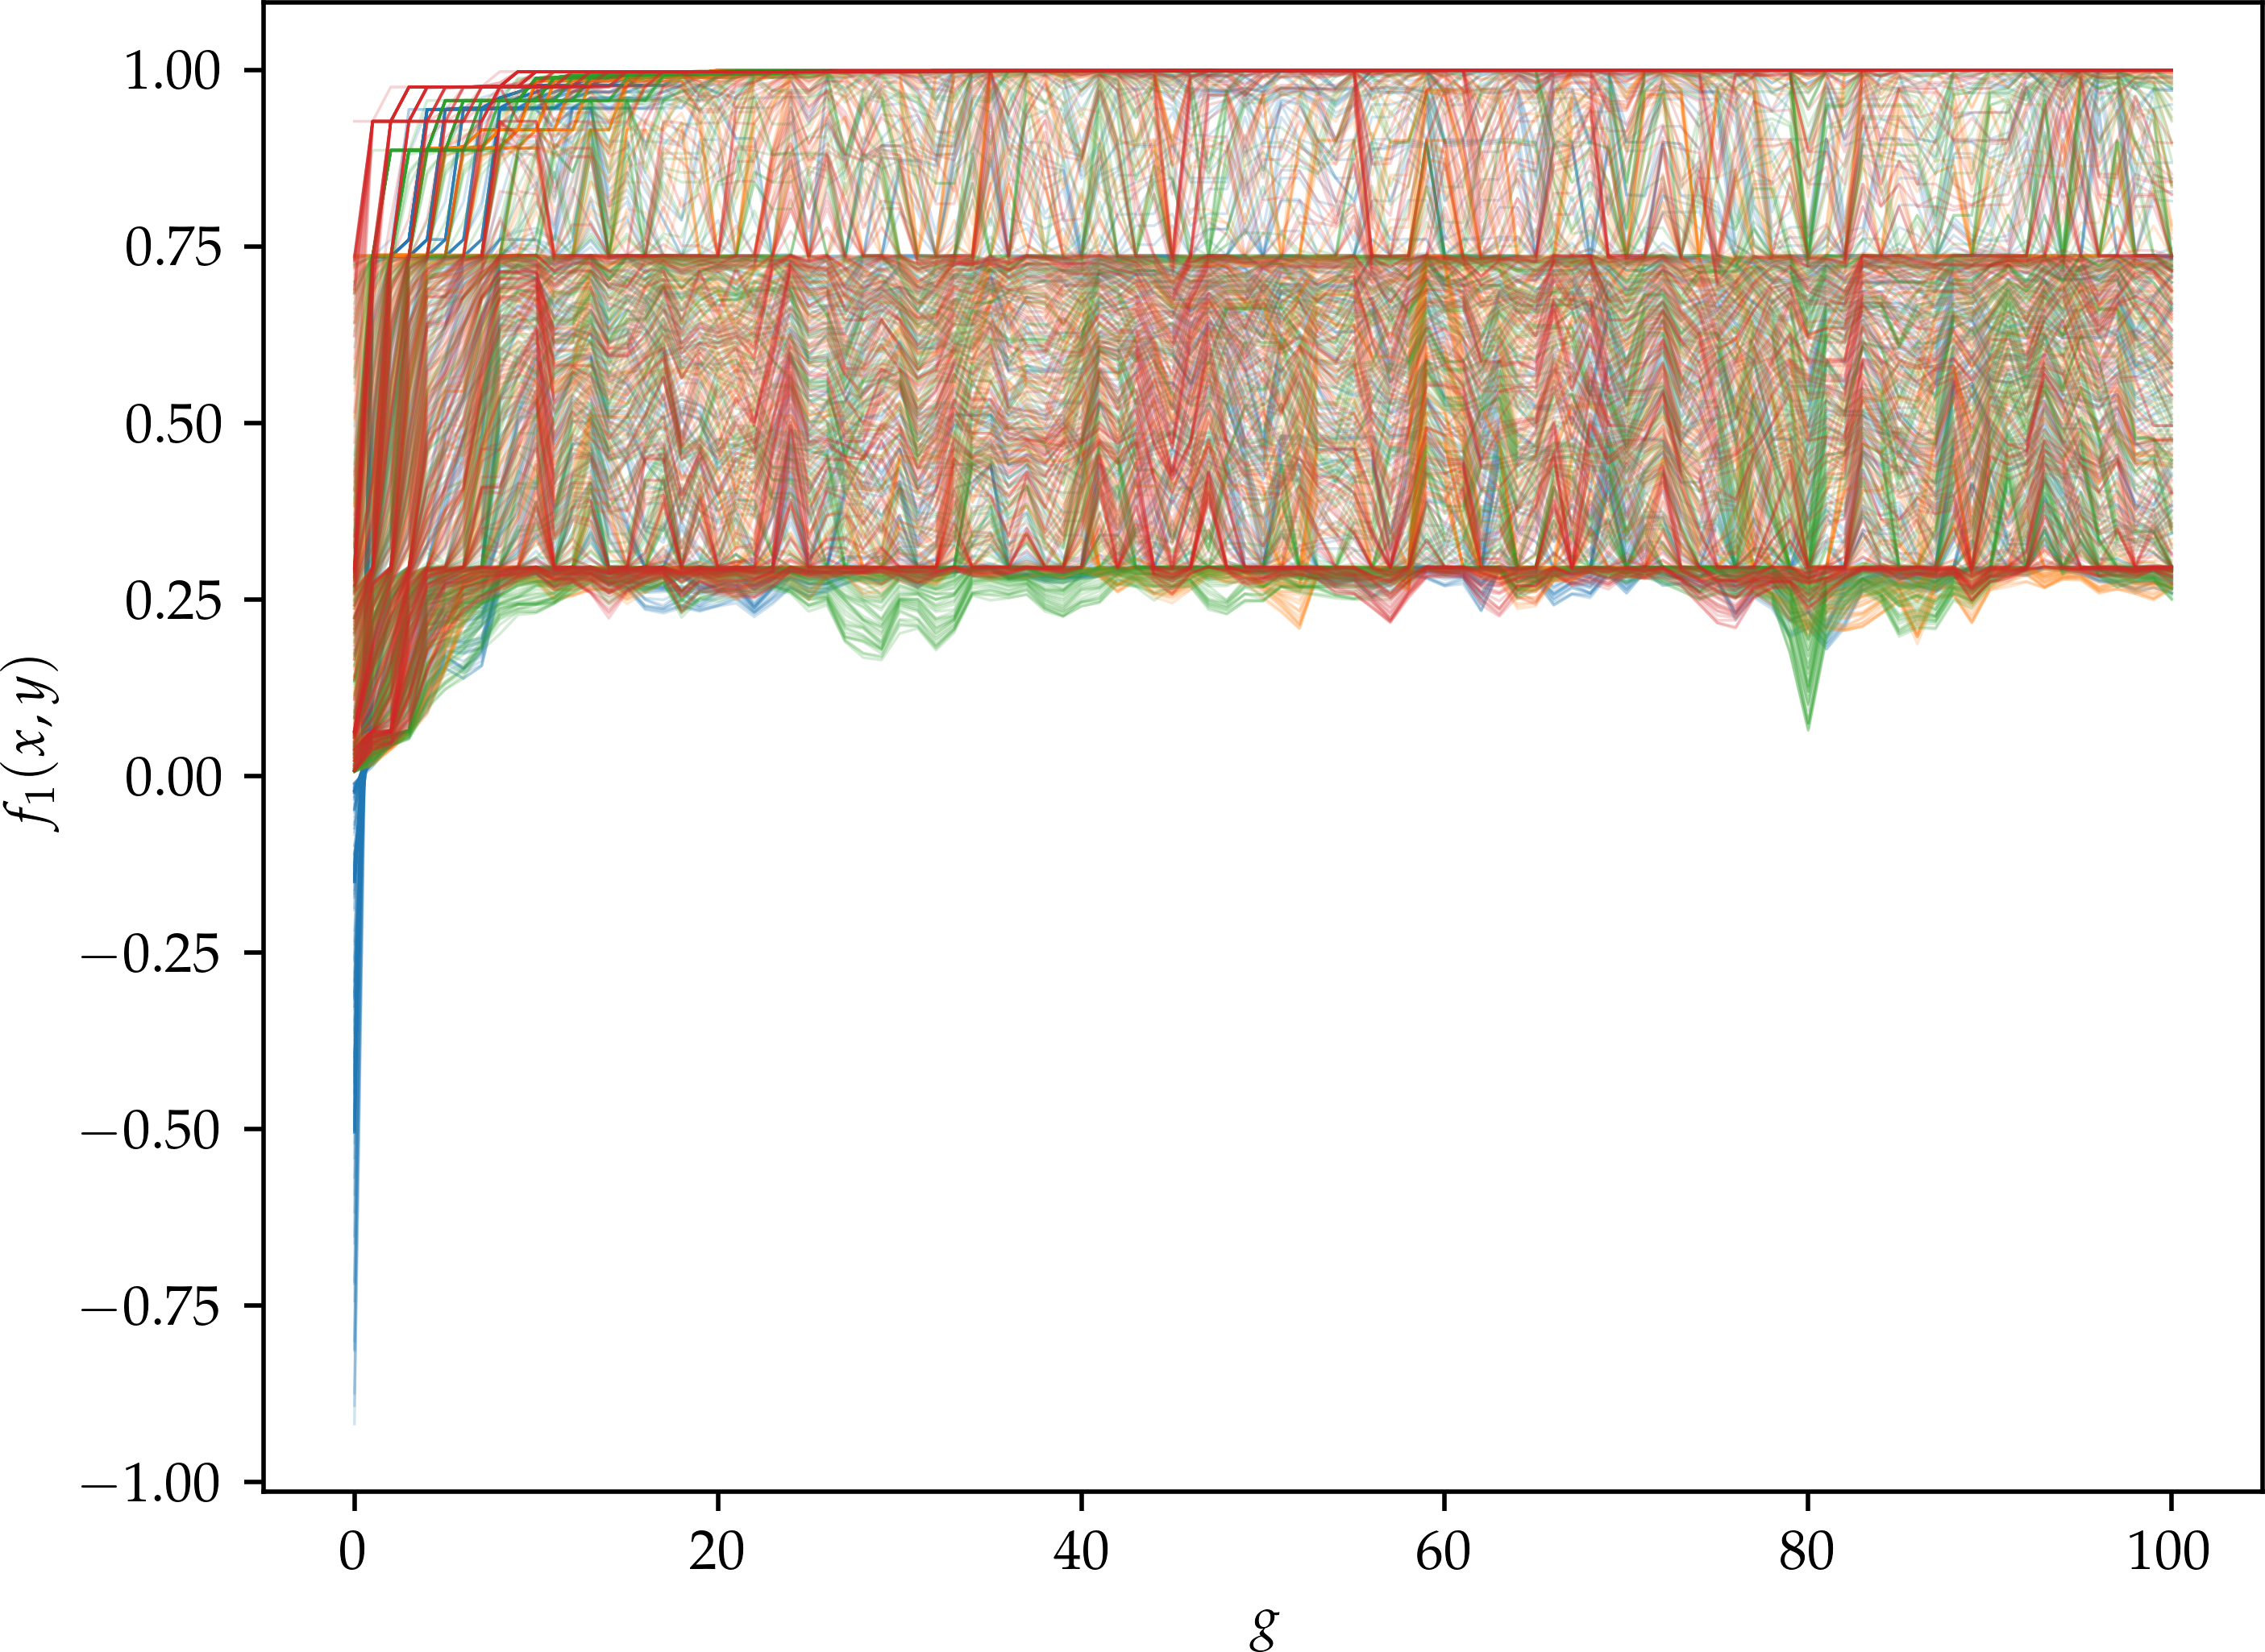
\includegraphics[height=0.95\textheight]{imagens/high_prob/evolution_damped_cossine.png}
  \end{figure}
\end{frame}

\begin{frame}
  \begin{figure}
    \centering
    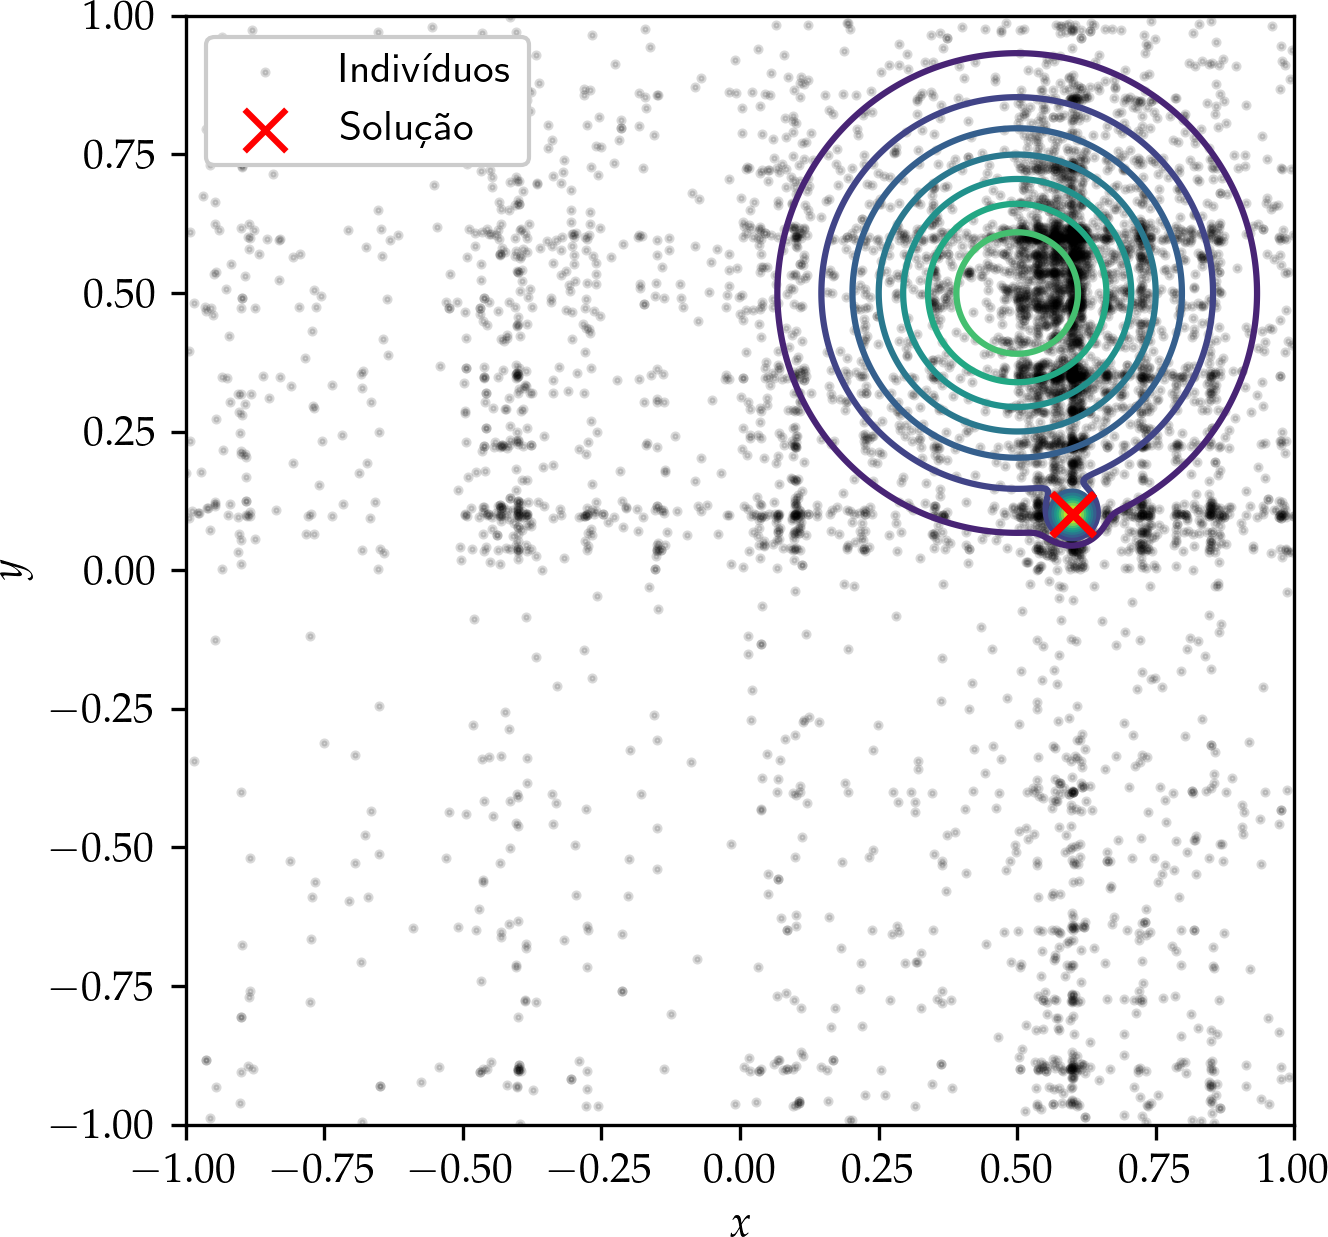
\includegraphics[height=0.95\textheight]{imagens/high_prob/contour_near_gaussians.png}
  \end{figure}
\end{frame}

\begin{frame}
  \begin{figure}
    \centering
    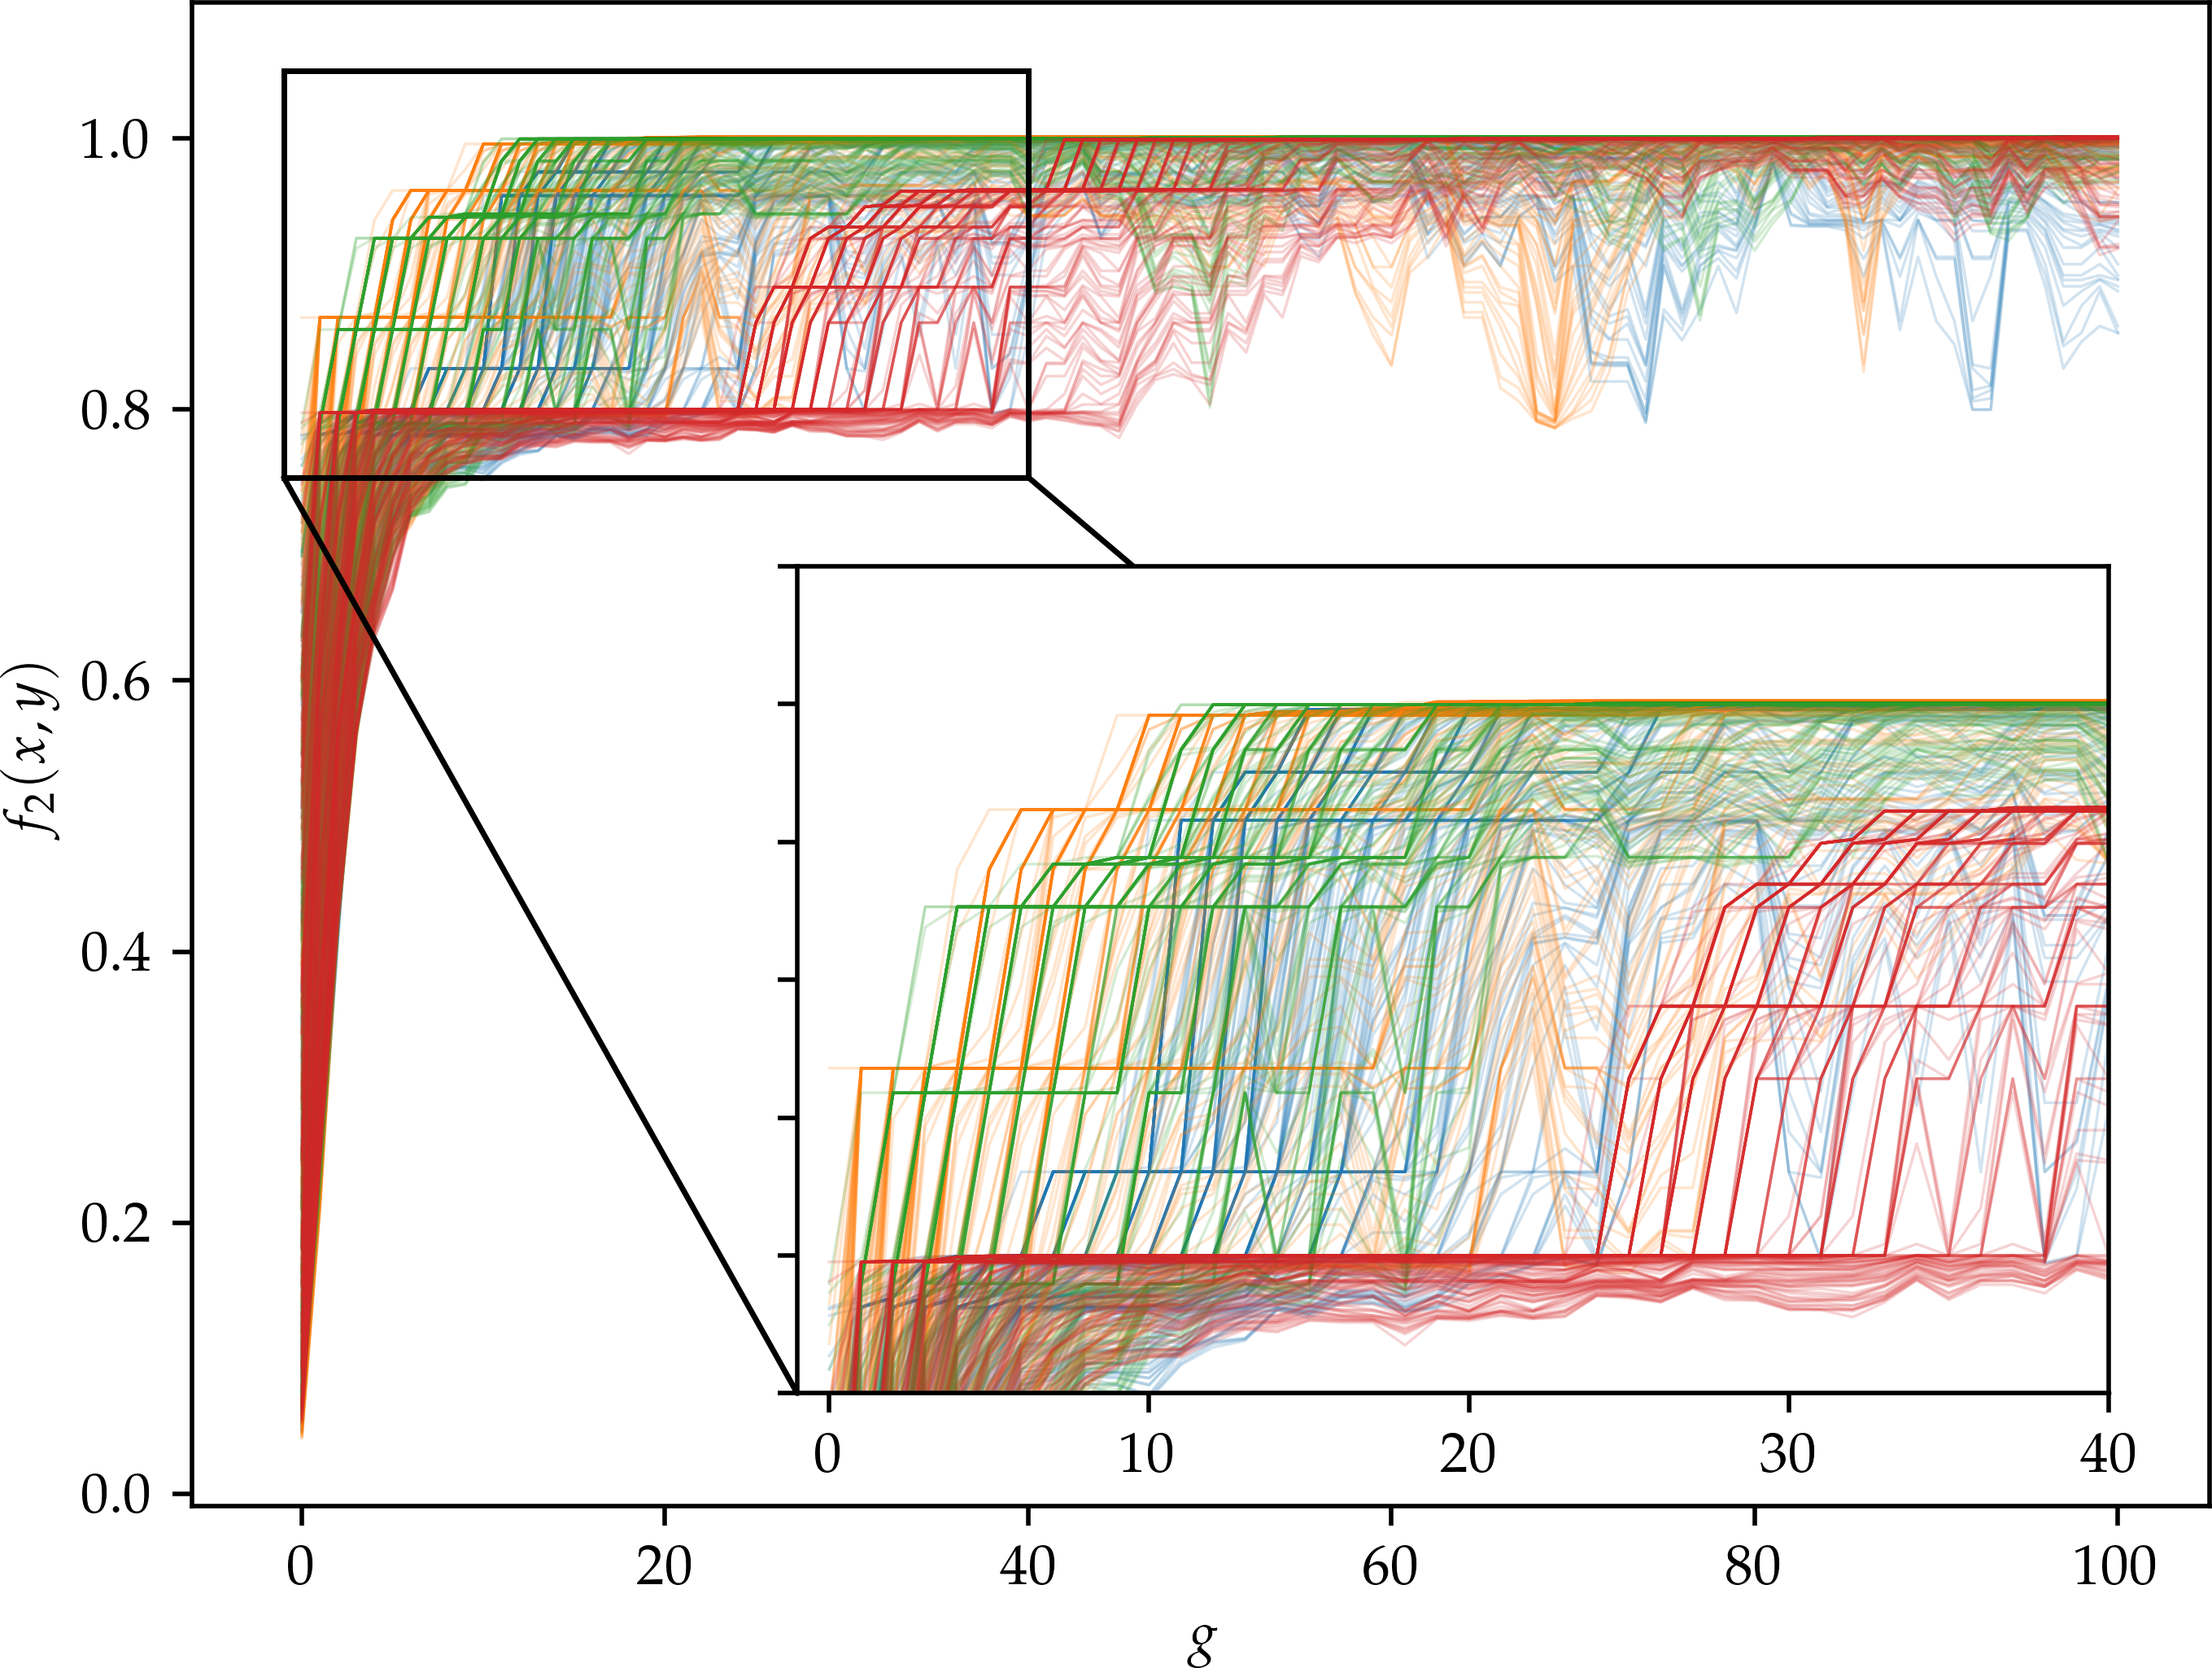
\includegraphics[height=0.95\textheight]{imagens/high_prob/evolution_near_gaussians.png}
  \end{figure}
\end{frame}

\begin{frame}
  \begin{block}{Conclusões}
    \begin{itemize}
      \item Em todos os casos o máximo global foi localizado
      \item Os máximos locais também foram localizados
      \item Uma variabilidade genética foi mantida
      \item A evolução por 100 gerações de 8 populações em paralelo
            levou $\approx$ 15 segundos
      \item Se mostrou escalável: 100 gerações com $10^5$ indivíduos
            em $\approx$ 1 hora
    \end{itemize}
  \end{block}
  \begin{alertblock}{O que não foi testado}
    \begin{itemize}
      \item Problemas com dimensão superior, como ajuste de curvas
            com 4 ou mais parâmetros
      \item Outros valores de $e_1$, $e_2$ e $e_3$
    \end{itemize}
  \end{alertblock}
\end{frame}

\bibliographystyle{abbrv}
\bibliography{bibliografia.bib}
\end{document}